\section{Introduction}

\begin{frame}{Introduction}
\begin{itemize}
    \item Block Cipher 
    \item XLS design 
    % (similar to SPN)
    \item It's security margins is similar with AES cipher 
    \item It has 4-bit S-boxes and 32-bit L-boxes and Shift Columns operation.
\end{itemize}
\end{frame}

\begin{frame}{Bit-Slicing}
    \begin{itemize}
        \item Converting the cipher into bit-wise operations (like the way we'd implement it in hardware)
        \item Carrying out those bit wise operations in parallel
    \end{itemize}
\end{frame}

\begin{frame}{XLS-Design}
\begin{itemize}
    \item LS Designs are a combination of linear diffusion L-boxes and non-linear bitslice S-boxes.
    \item These are  susceptible to invariant subspace attacks.
    \item So, XLS (eXtended LS) Designs model is developed by adding the Shiftcolumns operation to LS design models
    \item XLS-design comprises of SuperS-boxes, made of optimal components - 4-bit S-boxes and 32-bit L-boxes, and ShiftColumns operation.
\end{itemize}
\end{frame}

\begin{frame}{LS Design Model}


% \begin{figure}[H]
%      \centering
%     \subfloat[ls]{{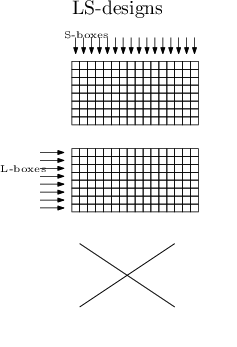
\includegraphics[width=4cm]{ls.png} }}%
%     % \qquad
%     % \subfloat[xls]{{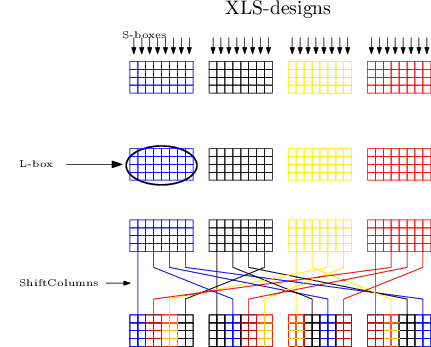
\includegraphics[width=4cm]{xls.png} }}%
    
%     \end{figure}
\begin{center}
    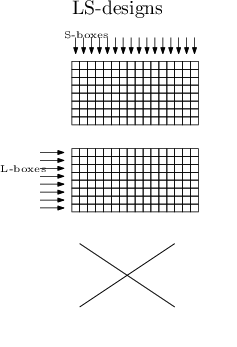
\includegraphics[width=4cm]{ls.png}
\end{center}

\end{frame}

\begin{frame}{XLS Design Model}
\begin{center}
    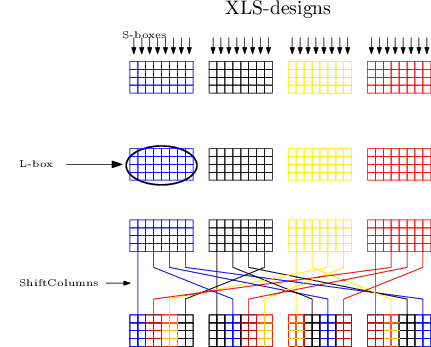
\includegraphics[width=5cm]{xls.png}
\end{center}
\end{frame}
